\subsection{The Identity on Real Data}
On SHAPE, the pre-stimulus mean of each z-scored epoch and channel correlates at $r=0.9965$ with $-m/\hat\sigma$ computed from the unscaled epoch (Fig.~\ref{fig:mechanism}c), as Proposition~\ref{prop:identity} predicts for a pre-stimulus window that approximates the baseline window. The two feature sets decode at BA 0.542 and 0.543 under the BIBM protocol, and their out-of-fold predictions agree on 95.9\% of observations. In microvolts the three conditions overlap before onset, and after z-scoring the neutral condition sits about 0.3 standard deviations above the two emotional conditions throughout the pre-stimulus interval (Fig.~\ref{fig:mechanism}a,b). This offset is the late positive potential of the emotional conditions \cite{hajcak2010lpp}, sign-flipped and moved to $t<0$.

\begin{figure*}[t]
\centering
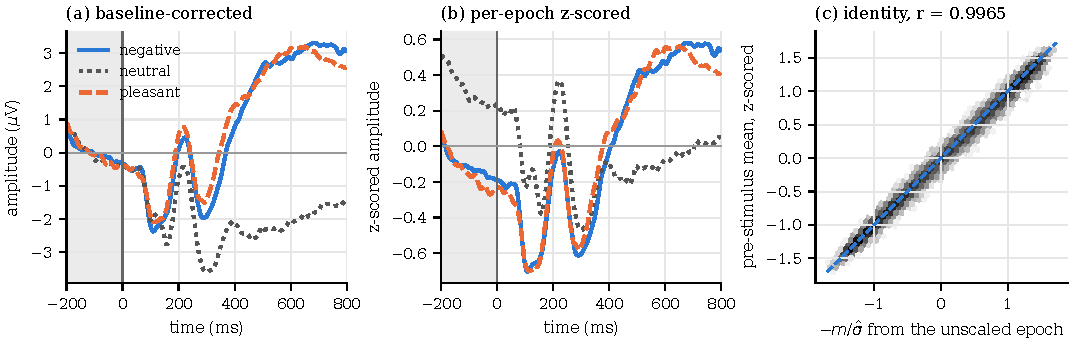
\includegraphics[width=\textwidth]{figures/fig_mechanism.pdf}
\caption{The leakage identity on SHAPE (211 participants, grand averages over participants and 34 channels). (a) Baseline-corrected ERPs overlap before onset (gray). (b) After per-epoch z-scoring the pre-stimulus interval is offset by condition. (c) Pre-stimulus mean of each z-scored epoch and channel against $-m/\hat\sigma$ of the unscaled epoch, log-density, $r=0.9965$ (dashed: identity line).}
\label{fig:mechanism}
\end{figure*}

\subsection{Pre-Stimulus Decoding on SHAPE}
Table~\ref{tab:shape} reports every encoder under every scaling. Under per-epoch z-scoring the 34 pre-stimulus channel means decode the three affective conditions at BA 0.542 [0.507, 0.575], against a within-participant permutation null with 95th percentile 0.371 and maximum 0.393 over 200 permutations. Under pre-stimulus scaling the same feature scores 0.346 [0.313, 0.381], inside its null (95th percentile 0.370). The paired difference between the two scalings is $+0.196$ [$+0.148$, $+0.242$] BA.

Time-resolved decoding locates the effect in time (Fig.~\ref{fig:shape}a). Under per-epoch z-scoring the first bin whose interval excludes chance is centered at $-193$~ms, the first bin of the epoch, and the mean pre-stimulus BA is 0.511. Under pre-stimulus scaling and under unscaled input the first such bin is centered at $+88$~ms, and the pre-stimulus means are 0.325 and 0.319. Z-scoring also attenuates the late structure that carries the genuine condition information: mean BA over 400 to 800~ms is 0.543 under z-scoring against 0.594 unscaled, with peaks of 0.602 and 0.632.

\begin{figure*}[t]
\centering
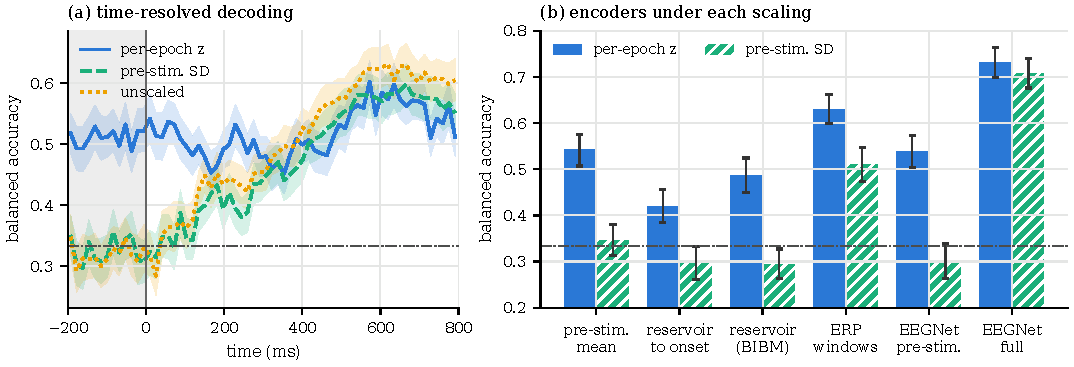
\includegraphics[width=\textwidth]{figures/fig_shape.pdf}
\caption{SHAPE, three affective conditions, chance $1/3$ (dash-dot). (a) Time-resolved decoding of the 34-channel pattern in 15.6~ms bins with participant-bootstrap 95\% intervals. Under per-epoch z-scoring decoding is above chance from the first pre-stimulus bin. (b) Balanced accuracy of each encoder under each scaling with participant-bootstrap 95\% intervals. The onset-truncated reservoir never receives a post-stimulus sample.}
\label{fig:shape}
\end{figure*}

\subsection{The ARSPI-Net Reservoir}
Under per-epoch z-scoring the BIBM reservoir configuration reproduces the published operating point exactly, BA 0.487 [0.450, 0.524] against the reported 0.487 [0.447, 0.523] \cite{lane2026bibm}, at a firing rate of 0.124. Under pre-stimulus scaling the same reservoir scores 0.294 [0.262, 0.327], and unscaled it scores 0.316 [0.278, 0.354]. The paired difference attributable to scaling is $+0.192$ [$+0.142$, $+0.243$] BA, which accounts for the full margin of the BIBM result above chance. The firing rate changes little between these scalings (0.124 to 0.144), so the difference does not come from a change in operating regime.

The onset-truncated reservoir isolates Corollary~\ref{cor:causal}. Its simulation stops at stimulus onset, so its spike counts are a function of pre-stimulus input alone. Driven by z-scored epochs it decodes at 0.420 [0.384, 0.457], and driven by pre-stimulus-scaled epochs at 0.297 [0.261, 0.333]. A causal dynamical system that has not yet received the stimulus therefore classifies the affective response to it, and the information enters through $m$ and $\hat\sigma$.

The ERP-window baseline of BIBM is affected as well, because its first window spans the pre-stimulus baseline. It scores 0.630 [0.599, 0.662] under z-scoring and 0.545 [0.512, 0.578] unscaled, a paired difference of $+0.085$ [$+0.049$, $+0.122$].
